\section{Stochastik}

\subsection{Baumdiagramm}

\boxx{Diagramm}{
    \begin{center}
        Aufgabe: Unter den Abonnenten sind $70\%$ höchstens $40$ Jahre als. Von diesen haben $80\%$ das Komplettpaket gewählt. Unter denjenigen Abonnenten, die älter sind als $40$ Jahre, haben sich $50\%$ für das Komplettpaket entschieden
    \end{center}

    \boxxline

    \begin{figure}[H] % Verhindert Gleitverhalten
        \centering
        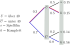
\includegraphics[width=0.8\linewidth]{figures/Baumdiagramm.pdf} % Pfad anpassen
    \end{figure}
}

\boxx{Pfadregel}{
        \begin{equation*}
            \text{\textcolor{graue}{Pfadregeln: }}\hspace{-0.2cm}\underbrace{P(U\cap s)}_{U40+\text{Spielfilm}}=0.3\cdot0.5=\hspace{-0.5cm}\underbrace{P_U(k)=\frac{2}{3}}_{\text{Komplettpaket für }U40}
        \end{equation*}
}

\boxx{Produktregel}{
    \begin{center}
        \crimson{Produktregel:} Wahrscheinlichkeit \crimson{einen bestimmten Versuchsausgang} zu erhalten, also die Wahrscheinlichkeit, dass eine Person über $40$ ist, und das Komplettpaket hat $0.3\cdot0.5=0.15$
    \end{center}
}

\boxx{Summenregel}{
    \begin{center}
        \blaue{Summenregel:} Wahrscheinlichkeit \blaue{mehrere Versuchsausgänge} zu erhalten, also die Wahrscheinlichkeit, dass das Komplettpaket gebucht wurde $0.3\cdot0.5+0.7\cdot0.8=0.71$
    \end{center}
}

\pagebreak

\subsection{Vierfeldertafel}

\boxx{Diagramm}{
    \begin{figure}[H] % Verhindert Gleitverhalten
        \centering
        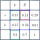
\includegraphics[width=0.5\linewidth]{figures/Vierfeldertafel.pdf} % Pfad anpassen
    \end{figure}
    \begin{center}
        Hilfe zur Berechnung von Ereignissen
    \end{center}
    \begin{equation*}
        \text{\textcolor{blaue}{geschnittene Wahrscheinlichkeit}}
    \end{equation*}
    \begin{equation*}
        \crimson{P(\overline{U}\cap s)}=0.14
    \end{equation*}
    \begin{center}
        \jade{bedingte Wahrscheinlichkeit}
        \begin{equation*}
            P_U(s)=\dfrac{P(U\cap s)}{P(U)}\qquad\frac{0.15}{0.3}=50\%
        \end{equation*}
        Leute die das Spiefilmpaket gekauft haben unter denen, die $40$ Jahre alt sind
    \end{center}
}

\subsection{Wahrscheinlichkeitsverteilung}

\boxx{Variablen}{
    \begin{center}
        \begin{tabularx}{\textwidth}{>{\centering\arraybackslash}X|>{\centering\arraybackslash}X}
            $n$ & Anzahl der ausgeführten Versuche oder Durchführungen \\
            \hline
            $p$ & Trefferwahrscheinlichkeit im Versuch \\
            \hline
            $X$ & Zufallsvariable \\
            \hline
            $\mu$ & Erwartungswert von $X$, $\mu=x_1\cdot P(X=x_1)+x_2\cdot P(X=x_2)+\dots$ \\
            \hline
            $\sigma$ & Standardabweichung von $X$, $\sigma=\sqrt{\left(x^1-\mu\right)^2\cdot P\left(X=x_1\right)+\dots}$ \\
        \end{tabularx}            
    \end{center}
}

\subsection{Bernoulli Versuch}

\boxx{Bernoulli-Formel}{
    \begin{equation*}
        P(X=k)=\binom{n}{k}\cdot p^k\cdot (1-p)^{n-k}\qquad\text{die Wahrscheinlichkeit für genau $k$ Erfolge in $n$ Versuchen}
    \end{equation*}
}

\boxx{Bernoullikoeffizient}{
    \begin{equation*}
        \binom{n}{k}\qquad\text{Anzahl, dass in $n$ Versuchen $k$ Erfolge eintreten}
    \end{equation*}
}

\boxx{Beispiel}{
    \begin{center}
        Es gibt drei Blutgruppen: O, A, B, AB. $41\%$ haben O. Es kommen $80$ Spender. 
    \end{center}
    \minipagee{0.5}{
        \begin{equation*}
            X=\text{Anzahl der Blutspender mit O}
        \end{equation*}
    }
    \minipagee{0.5}{
        \begin{align*}
            n&=80\\
            p&=0.41
        \end{align*}
    }
    
    \boxxline
    \vspace{\baselineskip}

    \minipagee{0.4}{
        \begin{itemize}
            \item Genau $25$ Spender haben O \begin{align*}
                P(X=25)&=1.9\%\\
                \text{binomPdf}(80;0.41;25)&=0.018917
            \end{align*}
            \item höchstens $20$ Spender haben O \begin{align*}
                P(X\leq20)&=0.2\%\\
                \text{binomCdf}(80;0.41;0;20)&=0.002061
            \end{align*}
            \item mindestens $30$ Spender haben O \begin{align*}
                P(X\geq30)&=72.2\%\\
                \text{binomCdf}(80;0.41;30;80)&=0.772405
            \end{align*}
        \end{itemize}
    }
}

\subsection{Kenngrößen}

\boxx{n}{
    \begin{center}
        Eine Maschine arbeitet nicht präzise. $3\%$ der Produkte sind mangelhaft. Wie viele Produkte müssen geprüft werden, dass mit $99\%$ Wahrscheinlichkeit ein Produkt mangelhaft ist?
    \end{center}
    \minipagee{0.5}{
        \begin{align*}
            X&=\text{Anzahl der mangelhaften Produkte}\\
            n&=?\\
            p&=0.03\qquad P(X\geq1)\geq99
        \end{align*}
    }
    \minipagee{0.5}{
        \begin{equation*}
            \dfrac{\ln(0.01)}{\ln(0.03)}=151.191\,\text{Produkte müssen geprüft werden}
        \end{equation*}
    }
}

\boxx{p}{    
    \begin{center}
        Ein Weihnachtskalender mit $24$ Türchen hat verschiedene Schokoladensorten. Was ist die Mindesterfolgswahrscheinlichkeit, mit der eine Sorte drin sein muss, sodass diese mit mindestens $95\%$ Wahrscheinlichkeit mindestens ein mal im Kalender ist?
    \end{center}
    \minipagee{0.5}{
        \begin{align*}
            X&=\text{Anzahl der Tafeln einer Sorte}\\
            n&=24
        \end{align*}
    }
    \minipagee{0.5}{
        \begin{equation*}
            1-\sqrt[24]{0.05}=0.117346\,\text{mit }11.8\%\text{ ist sie enthalten}
        \end{equation*}
    }
}

\boxx{k}{
    \begin{center}
        Für eine Studie wurden $500$ Personen genötigt. Nur $75\%$ der befragten wollen daran teilnehmen. Wie viele Personen müssen befragt werden, dass zu $95\%$ $500$ Leute zur Auskunft bereit werden?
    \end{center}
    \minipagee{0.5}{
        \begin{align*}
            X&=\text{Anzahl der befragten Personen}\\
            p&=0.75\\
            k&\geq500
        \end{align*}
    }
    \minipagee{0.5}{
        \begin{align*}
            \text{binomCdf}&(700;0.75;0;499)\\
            \text{binomCdf}&(690;0.75;0;499)\\
            \text{binomCdf}&(692;0.75;0;499)\\
            \text{binomCdf}&(692;0.75;500;592)=0.955
        \end{align*}
    }
}

\subsection{Mu und Sigma}

\boxx{Erwartungswert einer binomialverteilten Zufallsgröße}{
    \begin{equation*}
        \mu=n\cdot p
    \end{equation*}
}

\subsection{Standardabweichung}

\boxx{Standardabweichung einer binomialverteilten Zufallsgröße}{
    \begin{equation*}
        \sigma=\sqrt{n\cdot p\cdot (1-p)}
    \end{equation*}
}

\subsection{Normalverteilung}

\boxx{Beispiel}{
    \begin{center}
        Körpergrößen können näherungsweise mithilfe einer normalverteilten Zufallsgröße modelliert werden. Es ergibt sich für die Körpergröße von $18$ bis $20$-jährigen Frauen ein Mittelwert von $1.68$m bei einer Standardabweichung von $6.5$cm
    \end{center}
    \begin{center}
        $X=$Körpergröße $18$ bis $20$-jähriger Frauen\\
        $\mu=1.68$cm$\qquad\sigma=6.5$cm
    \end{center}
    \vspace{-\baselineskip}
    \begin{align*}
        \text{kleiner als }1.65=P(X<165)=\text{normCdf}(-\infty;165;168;6.5)=0.322206=32.22\%\\
        \text{größer als }1.80=P(X>180)=\text{normCdf}(180;+\infty;168;6.5)=0.032435=3.24\%\\
        \text{zwischen }1.70\text{ und }1.75=P(170\leq X\leq175)=\text{normCdf}(170;175;168;6.5)=0.238401=23.84\%\\
        \text{genau }1.70=P(X=170)=\text{normPdf}(170;168;6.5)=0.058538=5.85\%
    \end{align*}
}

\subsection{Sigmaregeln}

\boxx{$1\sigma,\,2\sigma,\,3\sigma$-Regel}{
    \begin{center}
        Für $\mu=n\cdot p$ und $\sigma=\sqrt{n\cdot p\cdot(1-p)}$ erhält man die Näherung
    \end{center}
    \vspace{-\baselineskip}
    \begin{align*}
        1.&P(\mu-\sigma\leq X\leq\mu+\sigma)=68.3\%\\
        2.&P(\mu-2\sigma\leq X\leq\mu+2\sigma)=95.4\%\\
        3.&P(\mu-3\sigma\leq X\leq\mu+3\sigma)=99.7\%
    \end{align*}
}

\boxx{"glatte" Wahrscheinlichkeiten}{
    \vspace{-\baselineskip}\begin{align*}
        4.&P(\mu-1.64\sigma\leq X\leq\mu+1.64\sigma)=90\%\\
        5.&P(\mu-1.96\sigma\leq X\leq\mu+1.96\sigma)=95\%\\
        6.&P(\mu-2.58\sigma\leq X\leq\mu+2.58\sigma)=99\%
    \end{align*}
}

\subsection{Hypothesentests}

\boxx{linksseitiger Hypothesentest}{
    \begin{center}
        Beispiel:\\
        Max hat einen Würfel $600$-mal geworfen und $87$ mal eine drei erhalten. Du hälst den Würfel für gezinkt. Führe einen linksseitigen Hypothesentest mit einem Signifikanzniveau $\alpha=5\%$ durch. Bestimme sein Ablehnungsbereich und gib eine Entschiedungsregel für dein Ergebnis an.
    \end{center}
    \vspace{-\baselineskip}
    \begin{align*}
        X&=\text{Anzahl der Dreien}\\
        n&=600\\
        p&=\dfrac{1}{6}\\
    \end{align*}
}

\boxx{Nullhypothese}{
    \begin{center}
        $H_0$: Der Würfel ist fair, $p=\dfrac{1}{6}$. Grenze des Ablehnungsbereichs $P(X\leq g)\leq0.05$
    \end{center}
}

\boxx{Alternative}{
    \begin{center}
        $H_1$: Der Würfel ist gezinkt, $p<\dfrac{1}{6}$. Grenze des Ablehnungsbereichs $P(X\leq g)\leq0.05$
    \end{center}
    \begin{center}
        \begin{tabular}{c|c}
            $g$&$P(X\leq g)$\\
            \hline
            $90$&$0.1487$\\
            $85$&$0.0538$\\
            $84$&$0.0424$ (Alpha Fehler)
        \end{tabular}
    \end{center}
    \begin{center}
        Ablehnungsbereich A$[0;84]\to$ hätte er weniger als $84$ gewürfelt wäre die Nullhypothese abgelehnt.
    \end{center}
}

\boxx{Alpha Fehler}{
    \begin{center}
        Wahrscheinlichkeit, dass die Aussage verworfen wird, obwohl man recht hat.
    \end{center}
}

\boxx{Beta Fehler}{
    \begin{center}
        Nullhypothese wird angenommen, obwohl sie abgelehnt hätte werden müssen
    \end{center}
    \vspace{-\baselineskip}
    \begin{align*}
        n&=600\\
        p&=\dfrac{1}{6}\\
    \end{align*}
    \begin{center}
        $0.045$ mit einer Wahrscheinlichkeit von $4\%$ ist der Würfel gezinkt, aber es wurde die falsche Probe genommen bei $84$.
    \end{center}
}